% Fig. 1 of the paper: the protocol for one query between two banks.
% Source of docs/paper/figures/fig_architecture.pdf (vector, fonts embedded). Rebuild with
%   cd docs/paper/static && pdflatex fig_architecture && mv fig_architecture.pdf ../figures/
% Every element is checked against the code in docs/paper/VERIFICATION.md ("Fig. 1" rows).
% Updated from the proposal's workflow diagram (docs/proposal/workflow.png) to the system
% that was built and evaluated.
\documentclass[10pt,border=0.5pt]{standalone}
\usepackage{times}
\usepackage{amsmath}
\usepackage{tikz}
\usetikzlibrary{positioning,calc,fit}

\begin{document}
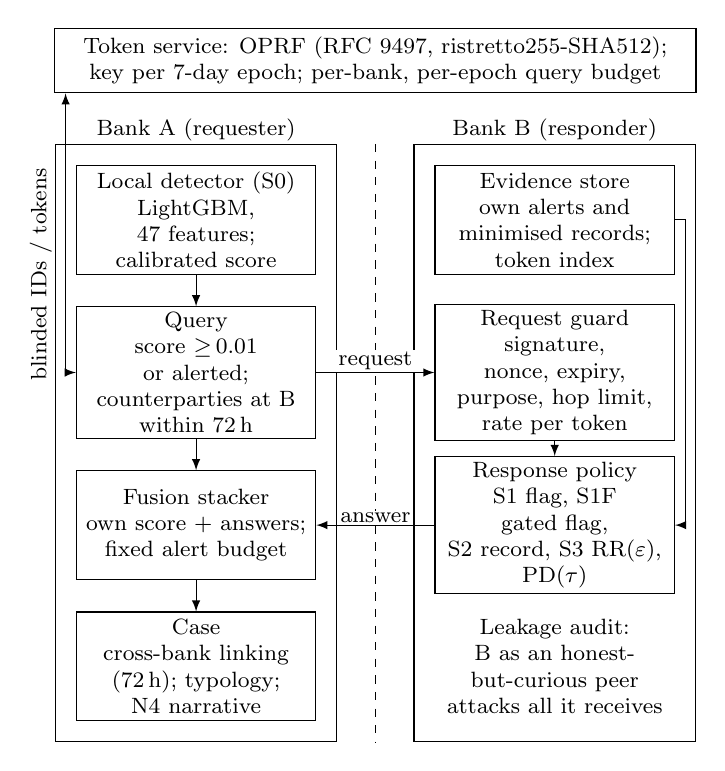
\begin{tikzpicture}[
  font=\footnotesize, >=latex,
  box/.style={draw, line width=0.4pt, align=center, text width=29mm, inner sep=2pt,
              minimum height=13.8mm},
  lbl/.style={align=center, inner sep=0.8pt},
  node distance=4mm and 15mm,
]
% bank A (requester)
\node[box] (a1) {Local detector (S0)\\ LightGBM, 47 features;\\ calibrated score};
\node[box, below=of a1] (a2) {Query\\ score ${\ge}\,0.01$ or alerted;\\ counterparties at B\\ within 72\,h};
\node[box, below=of a2] (a3) {Fusion stacker\\ own score + answers;\\ fixed alert budget};
\node[box, below=of a3] (a4) {Case\\ cross-bank linking\\ (72\,h); typology;\\ N4 narrative};

% bank B (responder)
\node[box, right=of a1] (b3) {Evidence store\\ own alerts and\\ minimised records;\\ token index};
\node[box, right=of a2] (b1) {Request guard\\ signature, nonce, expiry,\\ purpose, hop limit,\\ rate per token};
\node[box, right=of a3] (b2) {Response policy\\ S1 flag, S1F gated flag,\\ S2 record, S3 RR($\varepsilon$),\\ PD($\tau$)};
\node[lbl, text width=29mm] (aud) at (b2 |- a4) {Leakage audit: B as an honest-but-curious peer attacks all it receives};

% banks and boundary
\node[draw, line width=0.4pt, inner sep=2.6mm, fit=(a1)(a4)] (laneA) {};
\node[draw, line width=0.4pt, inner sep=2.6mm, fit=(b3)(b2)(aud)(b2 |- a4.south)] (laneB) {};
\node[lbl, anchor=south] (tA) at (laneA.north) {Bank A (requester)};
\node[lbl, anchor=south] at (laneB.north) {Bank B (responder)};
\path ($(laneA.north east)!0.5!(laneB.north west)$) coordinate (bt)
      ($(laneA.south east)!0.5!(laneB.south west)$) coordinate (bb);
\draw[dashed, line width=0.4pt] (bt) -- (bb);

% token service, spanning both banks
\path (laneA.north west) ++(0,6.5mm) coordinate (tsw);
\path (laneB.north east) ++(0,6.5mm) coordinate (tse);
\node[draw, line width=0.4pt, align=center, inner sep=2pt, fit={(tsw) (tse) ($(tse)+(0,8.2mm)$)},
      inner sep=0pt] (tsbox) {};
\node[lbl] at (tsbox.center) {Token service: OPRF (RFC 9497, ristretto255-SHA512);\\
   key per 7-day epoch; per-bank, per-epoch query budget};

% flow
\draw[->] (a1) -- (a2);
\draw[->] (a2) -- (a3);
\draw[->] (a3) -- (a4);
\draw[->] (b1) -- (b2);
\draw[->] (b3.east) -- ++(1.3mm,0) |- (b2.east);
\draw[->] (a2.east) -- node[lbl, above, fill=white] {request} (b1.west);
\draw[->] (b2.west) -- node[lbl, above, fill=white] {answer} (a3.east);

% tokens (blinded)
\draw[<->] (a2.west) -- ++(-1.3mm,0) coordinate (ta) -- (ta |- tsbox.south);
\node[lbl, rotate=90, anchor=south] at ($(laneA.west |- a1.south)$) {blinded IDs / tokens};
\end{tikzpicture}
\end{document}
